\documentclass[aps,prd,a4paper,preprint,preprintnumbers,titlepage,
nofootinbib,superscriptaddress]{revtex4-2}

\usepackage[a4paper, hdivide={1.91cm,,1.165cm},
vdivide={1.83cm,,3.0cm}]{geometry}
\usepackage[T1]{fontenc}
\usepackage[utf8]{inputenc}
\usepackage{amsmath,amssymb,mathtools}
\usepackage{bm}
\usepackage{booktabs}
\usepackage{graphicx}
\usepackage{xcolor}
\usepackage[colorlinks=true,linkcolor=blue,citecolor=blue,urlcolor=blue]{hyperref}

\allowdisplaybreaks[1]

\newcommand{\ii}{\mathrm{i}}
\newcommand{\Ds}{D_s}
\newcommand{\Dst}{D_s^\ast}
\newcommand{\Dsone}{D_{s1}}
\newcommand{\Bs}{B_s}
\newcommand{\Bst}{B_s^\ast}
\newcommand{\Bsone}{B_{s1}}
\newcommand{\GeV}{\mathrm{GeV}}
\newcommand{\MeV}{\mathrm{MeV}}
\newcommand{\keV}{\mathrm{keV}}
\newcommand{\qqbar}{\langle\bar q q\rangle}
\newcommand{\ssbar}{\langle\bar s s\rangle}
\newcommand{\gstar}{g^\ast}
\newcommand{\fgammas}{f_{\gamma,s}^{\perp}}
\providecommand{\orcidlink}[1]{}

\begin{document}

\title{Radiative transitions of strange heavy axial mesons into vector mesons in light-cone QCD sum rules}

\author{T.~M.~Aliev\,\orcidlink{0000-0001-8400-7370}}
\email{taliev@metu.edu.tr}
\affiliation{Department of Physics, Middle East Technical University,
Ankara, 06800, Turkey}

\author{S.~Bilmis\,\orcidlink{0000-0002-0830-8873}}
\email{sbilmis@metu.edu.tr}
\affiliation{Department of Physics, Middle East Technical University,
Ankara, 06800, Turkey}
\affiliation{TUBITAK ULAKBIM, Ankara, 06510, Turkey}

\author{M.~Savci\,\orcidlink{0000-0002-6221-4595}}
\email{savci@metu.edu.tr}
\affiliation{Department of Physics, Middle East Technical University,
Ankara, 06800, Turkey}

\date{\today}

\begin{abstract}
We calculate the radiative transitions
\(\Dsone(2460)\to\Dst\gamma\),
\(\Dsone(2536)\to\Dst\gamma\),
\(B_{s1}(5750)\to\Bst\gamma\), and
\(\Bsone(5830)\to\Bst\gamma\)
in light-cone QCD sum rules.  The calculation is performed for the two
independent axial-vector basis currents and the physical amplitudes are
obtained by applying the same mixing convention as in the two-point
normalization.  The \(J_\mu^B\) tensor-current contribution is included through
the soft photon-distribution-amplitude terms and a calibrated hard-photon
spectral density.  With the lattice-normalized leading-twist strange-photon
input and fixed \(\theta=35.3^\circ\), we find
\(\Gamma[\Dsone(2460)\to\Dst\gamma]=92.3^{+46.4}_{-32.6}~\keV\) and
\(\Gamma[\Dsone(2536)\to\Dst\gamma]=23.0^{+12.1}_{-6.5}~\keV\).
For the bottom-strange channels we obtain
\(\Gamma[B_{s1}(5750)\to\Bst\gamma]=10.2^{+6.0}_{-3.6}~\keV\) and
\(\Gamma[\Bsone(5830)\to\Bst\gamma]=7.46^{+16.5}_{-4.16}~\keV\).
The charm-strange vector-final-state widths are compatible with the
constructive/destructive interference pattern emphasized in recent
phenomenological analyses, while the bottom-strange widths remain predictions
for future radiative searches.
\end{abstract}

\keywords{radiative transitions; strange heavy mesons; light-cone QCD sum rules; photon distribution amplitudes}
\maketitle

\section{Introduction}
\label{sec:intro}

Radiative decays of positive-parity strange heavy mesons probe both the
spin composition of the initial axial-vector state and the electromagnetic
structure of the light and heavy quark lines.  They are therefore a useful
complement to mass spectroscopy and strong-decay measurements.  The
charm-strange mesons \(\Dsone(2460)\) and \(\Dsone(2536)\) are especially
interesting because they are narrow and because the two physical \(1^+\)
states are mixtures of the two axial configurations that become
\({}^3P_1\) and \({}^1P_1\) in the quark-model language.

The radiative modes with a pseudoscalar final meson,
\(\Dsone\to\Ds\gamma\), have been studied in light-cone QCD sum rules
(LCSR), quark models, and phenomenological approaches
\cite{Goity:2000dk,Godfrey:2005ww,Colangelo:2005hv,Radford:2009bs,
Green:2016occ,Chen:2020ejk,Bondar:2023mua,Bondar:2025smw}.  The vector
final-state modes,
\(\Dsone\to\Dst\gamma\), are equally important because they test a different
Lorentz structure and a different final-state decay constant.  They also
appear in the comparison tables collected by Bondar and Milstein
\cite{Bondar:2025smw}, where a pronounced hierarchy between the two
charm-strange axial states is explained by the relative sign of the two mixed
spin components.  The corresponding bottom-strange channels
\(\Bsone\to\Bst\gamma\) are experimentally unexplored and provide useful
predictions for future searches.

Experimentally, \(\Dsone(2460)\) is observed in radiative and isospin-violating
channels, and BaBar measured the branching fractions for
\(\Dsone(2460)\to\Ds\gamma\) and \(\Dsone(2460)\to\Dst\pi^0\)
\cite{BaBar:2006eep}.  There is, however, no direct partial-width measurement
for \(\Dsone(2460)\to\Dst\gamma\).  The \(\Dsone(2536)\) total width is
measured to be \(0.92\pm0.03\pm0.04~\MeV\) by BaBar
\cite{BaBar:2011zpy}, but its radiative partial widths are not directly
measured.  In the bottom-strange sector, \(\Bsone(5830)\) is observed in
\(B^{(*)}K\) spectroscopy \cite{CMS:2018qdl}; there is no direct information
on the radiative \(\Bst\gamma\) modes.

In this work we extend the LCSR analysis to the vector-final-state transitions
\[
  \Dsone(2460,2536)\to\Dst\gamma,\qquad
  B_{s1}(5750),\Bsone(5830)\to\Bst\gamma .
\]
The lower bottom-strange state is treated as a theoretical diagnostic rather
than as an experimentally established resonance.  We keep the strange-quark
mass terms, use photon distribution amplitudes in the BBK/Rohrwild convention
\cite{Ball:2002ps,Rohrwild:2007yt}, and compare the conventional
susceptibility normalization with the recent lattice normalization of the
leading-twist strange-photon matrix element \cite{Bacchio:2024pij}.  The
central predictions quoted below use the lattice-normalized input
\(\fgammas(1~\GeV)=-55.1(1.9)~\MeV\).

The paper is organized as follows.  In Sec.~\ref{sec:framework} we define the
currents, form factor, width formula, and basis-current sum rules.  In
Sec.~\ref{sec:numerics} we give the numerical inputs, stability-window
discussion, final results, no-mixing benchmark, and comparison with previous
work and experiment.  Section~\ref{sec:concl} summarizes the conclusions.

\section{Theoretical framework}
\label{sec:framework}

We consider the transition of an axial-vector strange heavy meson \(X\) with
momentum \(P=p+q\) and polarization vector \(\eta_\mu\) into a vector meson
\(V=\Dst,\Bst\), with momentum \(p\) and polarization vector \(\xi_\nu\), and
a real photon with momentum \(q\) and polarization vector \(\varepsilon_\rho\).
The heavy quark is denoted by \(Q=c,b\), and the light quark is \(s\).
The final vector current is
\begin{equation}
  j_\nu^V=\bar s\gamma_\nu Q,\qquad
  \langle0|j_\nu^V|V(p,\xi)\rangle=m_V f_V\xi_\nu .
  \label{eq:vector-current}
\end{equation}

For the initial axial-vector channel we use the two basis currents
\begin{align}
  J_\mu^A &= \bar s\gamma_\mu\gamma_5 Q,\\
  J_\mu^B &= \frac{\ii}{m_Q+m_s}\,
  \bar s\sigma_{\mu\alpha}P^\alpha\gamma_5 Q ,
  \label{eq:basis-currents}
\end{align}
where \(P^\alpha\) is the momentum of the initial axial-vector meson.  The
physical-current combinations are
\begin{align}
  J_{1\mu} &= \sin\theta\,J_\mu^A+\cos\theta\,J_\mu^B,\\
  J_{2\mu} &= \cos\theta\,J_\mu^A-\sin\theta\,J_\mu^B .
  \label{eq:physical-currents}
\end{align}
The lower state is coupled to \(J_{1\mu}\), while the higher state is coupled
to \(J_{2\mu}\).  Thus \(J_1\) is assigned to \(\Dsone(2460)\) and
\(B_{s1}(5750)\), and \(J_2\) to \(\Dsone(2536)\) and \(\Bsone(5830)\).
The decay constants of the physical currents are defined by
\begin{equation}
  \langle0|J_{i\mu}|X_i(P,\eta)\rangle=f_i m_i\eta_\mu,\qquad i=1,2 .
  \label{eq:physical-decay-constants}
\end{equation}

The \(1^+\to1^-\gamma\) matrix element is parametrized by
\begin{equation}
  \langle V(p,\xi)\gamma(q,\varepsilon)|X(P,\eta)\rangle
  =
  \ii e\,\gstar\,
  \epsilon_{\alpha\beta\rho\sigma}
  \eta^\alpha \xi^{\ast\beta}\varepsilon^{\ast\rho}q^\sigma .
  \label{eq:matrix-element}
\end{equation}
With this convention \(\gstar\) is dimensionless.  The corresponding partial
width is
\begin{equation}
  \Gamma(X\to V\gamma)
  =
  4\pi\alpha_{\rm em}
  \frac{m_X^2-m_V^2}{16\pi m_X^3}
  \frac{(m_X^2-m_V^2)^2(m_X^2+m_V^2)}{6m_X^2m_V^2}
  |\gstar|^2 .
  \label{eq:width}
\end{equation}

The vacuum-to-photon correlation function for a basis current is
\begin{equation}
  \Pi_{\mu\nu}^K(p,q)=\ii\int d^4x\,e^{\ii p\cdot x}
  \langle\gamma(q,\varepsilon)|
  T\{\bar s(x)\gamma_\nu Q(x)\,\bar Q(0)\Gamma_\mu^K s(0)\}
  |0\rangle ,
  \qquad K=A,B ,
  \label{eq:correlator}
\end{equation}
where \(\Gamma_\mu^A=\gamma_\mu\gamma_5\) and
\(\Gamma_\mu^B=\ii\sigma_{\mu\alpha}P^\alpha\gamma_5/(m_Q+m_s)\).  We
project the invariant amplitude multiplying
\begin{equation}
  \epsilon_{\mu\nu\rho\sigma}\varepsilon^\rho q^\sigma .
  \label{eq:epsilon-structure}
\end{equation}
The hadronic representation of the invariant amplitude contains the double
pole
\begin{equation}
  \Pi_K^{\rm had}(p^2,P^2)=
  \frac{m_X f_K\,m_V f_V\,G_K^\ast}
  {(m_X^2-P^2)(m_V^2-p^2)}
  +\cdots ,
  \qquad K=A,B ,
  \label{eq:hadronic-basis}
\end{equation}
where \(G_K^\ast\) denotes the basis-current form factor extracted before
the physical-current rotation.  In the physical basis the residue-weighted
rotation gives
\begin{align}
  f_1 g_1^\ast &=
  \sin\theta\,f_A G_A^\ast+\cos\theta\,f_B G_B^\ast,
  \label{eq:rotation-low}\\
  f_2 g_2^\ast &=
  \cos\theta\,f_A G_A^\ast-\sin\theta\,f_B G_B^\ast .
  \label{eq:rotation-high}
\end{align}
This form is used numerically; it is also the clean way to compare with the
no-mixing pure-current limit.

On the QCD side the heavy-quark propagator is used in the external
electromagnetic field.  In momentum representation,
\begin{align}
  S_Q(k) &=
  \frac{\not k+m_Q}{m_Q^2-k^2}
  -e_Q\int_0^1du
  \left[
  \frac{\not k+m_Q}{2(m_Q^2-k^2)^2}
  F^{\alpha\beta}(ux)\sigma_{\alpha\beta}
  +\frac{u x_\alpha F^{\alpha\beta}(ux)\gamma_\beta}{m_Q^2-k^2}
  \right]\notag\\
  &\quad
  -g_s\int_0^1du
  \left[
  \frac{\not k+m_Q}{2(m_Q^2-k^2)^2}
  G^{\alpha\beta}(ux)\sigma_{\alpha\beta}
  +\frac{u x_\alpha G^{\alpha\beta}(ux)\gamma_\beta}{m_Q^2-k^2}
  \right]+\cdots .
  \label{eq:heavy-propagator}
\end{align}
The photon emission from the light quark is represented by the standard
vacuum-to-photon matrix elements of nonlocal quark and quark-gluon operators.
We keep the terms proportional to \(m_s\) and use the photon distribution
amplitudes summarized in Appendix~\ref{app:details}.

After the double Borel transformation, we use the symmetric choice
\begin{equation}
  M_1^2=M_2^2=2M^2,\qquad
  u_0=\frac{M_1^2}{M_1^2+M_2^2}=\frac12 .
  \label{eq:borel-choice}
\end{equation}
The axial basis-current form factor is obtained from the published
Colangelo--De Fazio--Ozpineci spectral density and photon-DA terms
\cite{Colangelo:2005hv}, translated to our sign convention for
\(\chi_s\).  The tensor basis-current contribution is written as
\begin{equation}
  G_B^\ast=G_{B,{\rm soft}}^\ast+G_{B,{\rm hard}}^\ast .
  \label{eq:gb-split}
\end{equation}
The soft part comes from the photon-DA projection of the tensor-current
correlator.  The hard part is implemented through a calibrated spectral
density:
\begin{equation}
  \rho_B^{\rm hard}(s)
  =
  R_s^{\rm hard}(s)\rho_{A,s}^{\rm hard}(s)
  +R_Q^{\rm hard}(s)\rho_{A,Q}^{\rm hard}(s),
  \label{eq:calibrated-rho}
\end{equation}
where \(\rho_{A,s}^{\rm hard}\) and \(\rho_{A,Q}^{\rm hard}\) are the
strange-line and heavy-line pieces of the known axial hard density.  The
ratios \(R_s^{\rm hard}\) and \(R_Q^{\rm hard}\) are obtained from the
FeynCalc triangle reduction after removing the \(p\cdot q\) and
\(1/(p\cdot q)\) artifacts that cancel in the fully reduced axial benchmark.
This construction is therefore a calibrated hard-density implementation,
with the axial spectral density used as the normalization and sign check.

\section{Numerical analysis}
\label{sec:numerics}

\subsection{Inputs and working windows}
\label{subsec:inputs}

The numerical inputs are summarized in Table~\ref{tab:inputs}.  The vector
decay constants \(f_{\Dst}\) and \(f_{\Bst}\) are not assumed from external
models; they are calculated with a leading-order vector-current two-point
baseline and assigned conservative uncertainties from the Borel-window
envelope.  We obtain
\[
  f_{\Dst}=0.2270\pm0.0280~\GeV,\qquad
  f_{\Bst}=0.2615\pm0.0336~\GeV .
\]
The central mixing angle is \(\theta=35.3^\circ\).  We quote the fixed-angle
result as the headline comparison because the literature table of
Ref.~\cite{Bondar:2025smw} uses a fixed mixing convention; the
\(25^\circ\le\theta\le45^\circ\) scan is kept as a systematic diagnostic.

\begin{table}[t]
\centering
\caption{Main numerical inputs.  The photon-DA normalizations are quoted at
\(\mu=1~\GeV\).}
\label{tab:inputs}
\begin{ruledtabular}
\begin{tabular}{ll}
Parameter & Value and source\\
\colrule
\(m_c,\ m_b,\ m_s\) &
\(1.27(2),\ 4.18(3),\ 0.093(11)~\GeV\)
\cite{ParticleDataGroup:2024cfk}\\
\(M_{\Dsone(2460)},M_{\Dsone(2536)},m_{\Dst}\) &
\(2.4595,\ 2.53511,\ 2.1122~\GeV\)
\cite{ParticleDataGroup:2024cfk}\\
\(M_{\Bsone(5830)},m_{\Bst}\) &
\(5.82870,\ 5.4154~\GeV\)
\cite{ParticleDataGroup:2024cfk,CMS:2018qdl}\\
\(M_{B_{s1}(5750)}\) &
\(5.750(26)~\GeV\), diagnostic lower state\\
\(f_{\Dst}, f_{\Bst}\) &
\(0.2270(280),\ 0.2615(336)~\GeV\), this work\\
\(f_A(\Dsone), f_T(\Dsone)\) &
\(0.225(25),\ 0.256(17)~\GeV\)\\
\(f_A(B_{s1}), f_T(B_{s1})\) &
\(0.305(27),\ 0.285(27)~\GeV\) \cite{Pullin:2021ebn}\\
\(\chi_s(1~\GeV)\) &
\(+3.15(30)~\GeV^{-2}\) \cite{Rohrwild:2007yt}\\
\(\fgammas(1~\GeV)\) &
\(-55.1(1.9)~\MeV\) \cite{Bacchio:2024pij}\\
\end{tabular}
\end{ruledtabular}
\end{table}

The final windows are listed in Table~\ref{tab:windows}.  For the bottom
channels the continuum thresholds are above the pole masses by about
\(0.3\)--\(0.6~\GeV\), which is the expected location of the effective
continuum in a heavy-light sum rule.  The diagnostic scan gives very small
three-particle fractions, good tensor-channel pole proxies, and improved
width stability when the Borel interval is narrowed from \(8\le M^2\le14\)
to \(10\le M^2\le14~\GeV^2\).  The axial pole proxy is moderate in the
bottom sector, so we describe the windows as acceptable and stable rather
than strongly pole dominated.

\begin{table}[t]
\centering
\caption{Borel and continuum-threshold windows used in the final analysis.}
\label{tab:windows}
\begin{ruledtabular}
\begin{tabular}{lll}
Channel & \(M^2\) window & \(s_0\) window\\
\colrule
\(\Dsone(2460),\Dsone(2536)\to\Dst\gamma\) &
\(3.0\)--\(4.5~\GeV^2\) & \(7.5\)--\(8.5~\GeV^2\)\\
\(B_{s1}(5750)\to\Bst\gamma\) &
\(10.0\)--\(14.0~\GeV^2\) & \(36.5\)--\(40.5~\GeV^2\)\\
\(\Bsone(5830)\to\Bst\gamma\) &
\(10.0\)--\(14.0~\GeV^2\) & \(38.0\)--\(41.0~\GeV^2\)\\
\end{tabular}
\end{ruledtabular}
\end{table}

\subsection{No-mixing benchmark}
\label{subsec:no-mixing}

Before using the mixed physical currents, we check the pure-current limit.
This is the relevant comparison to same-method LCSR calculations: one sets
the physical mixing aside and compares the basis-current result with the
corresponding pure axial-current calculation.  For
\(\Dsone\to\Dst\gamma\) we find
\[
  G_A^\ast=-0.192\ldots -0.141 ,
\]
using Colangelo-like inputs and the original LCSR window.  The published
benchmark is \(g^\ast=-0.18\ldots -0.13\) \cite{Colangelo:2005hv}.  Thus the
sign and normalization of the axial-current vector-final-state sum rule are
reproduced.  For the pseudoscalar channel, the analogous pure-current check
gives \(g_1=[-0.344,-0.245]~\GeV^{-1}\), to be compared with the
Colangelo result \(g_1=[-0.37,-0.29]~\GeV^{-1}\).  This confirms that the
differences in the final mixed-state predictions are not caused by a basic
normalization error.

\subsection{Final results}
\label{subsec:results}

The final Monte Carlo results are listed in Table~\ref{tab:final-results}.
The table uses the preferred lattice photon normalization and fixed
\(\theta=35.3^\circ\).  The intervals are \(16\)--\(84\) percentile ranges.

\begin{table}[t]
\centering
\caption{Final vector-final-state predictions with the lattice-normalized
photon input and fixed \(\theta=35.3^\circ\).}
\label{tab:final-results}
\begin{ruledtabular}
\begin{tabular}{lcc}
Channel & \(g^\ast\) & \(\Gamma~(\keV)\)\\
\colrule
\(\Dsone(2460)\to\Dst\gamma\) &
\(-1.704\,[-2.083,-1.367]\) &
\(92.3\,[59.7,138.7]\)\\
\(\Dsone(2536)\to\Dst\gamma\) &
\(+0.654\,[0.554,0.808]\) &
\(23.0\,[16.5,35.1]\)\\
\(B_{s1}(5750)\to\Bst\gamma\) &
\(-1.383\,[-1.727,-1.138]\) &
\(10.2\,[6.63,16.24]\)\\
\(\Bsone(5830)\to\Bst\gamma\) &
\(+0.872\,[0.583,1.561]\) &
\(7.46\,[3.30,24.0]\)\\
\end{tabular}
\end{ruledtabular}
\end{table}

The corresponding angle-scan medians are
\[
  \Gamma[\Dsone(2460)\to\Dst\gamma]=93.1~\keV,\qquad
  \Gamma[\Dsone(2536)\to\Dst\gamma]=22.3~\keV,
\]
and
\[
  \Gamma[B_{s1}(5750)\to\Bst\gamma]=11.5~\keV,\qquad
  \Gamma[\Bsone(5830)\to\Bst\gamma]=2.55~\keV .
\]
The larger angle sensitivity in the high bottom-strange channel comes from
the same cancellation-sensitive physical-current normalization that appeared
in the pseudoscalar-final-state analysis.

\begin{figure}[t]
\centering
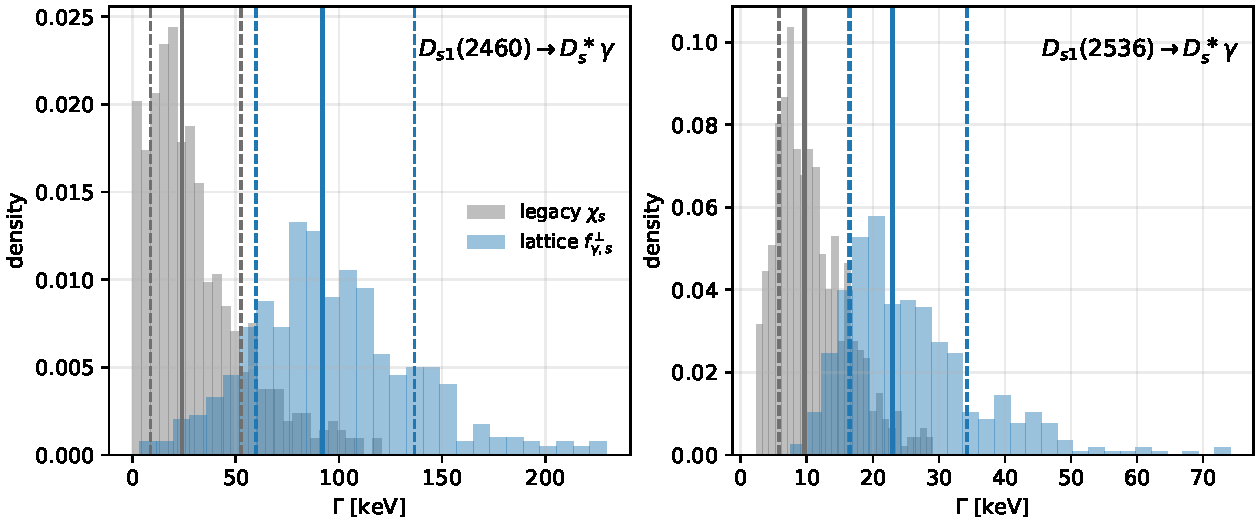
\includegraphics[width=0.48\textwidth]{../Dsstar_gamma/outputs/tensor_full_calibrated_monte_carlo_histograms.pdf}
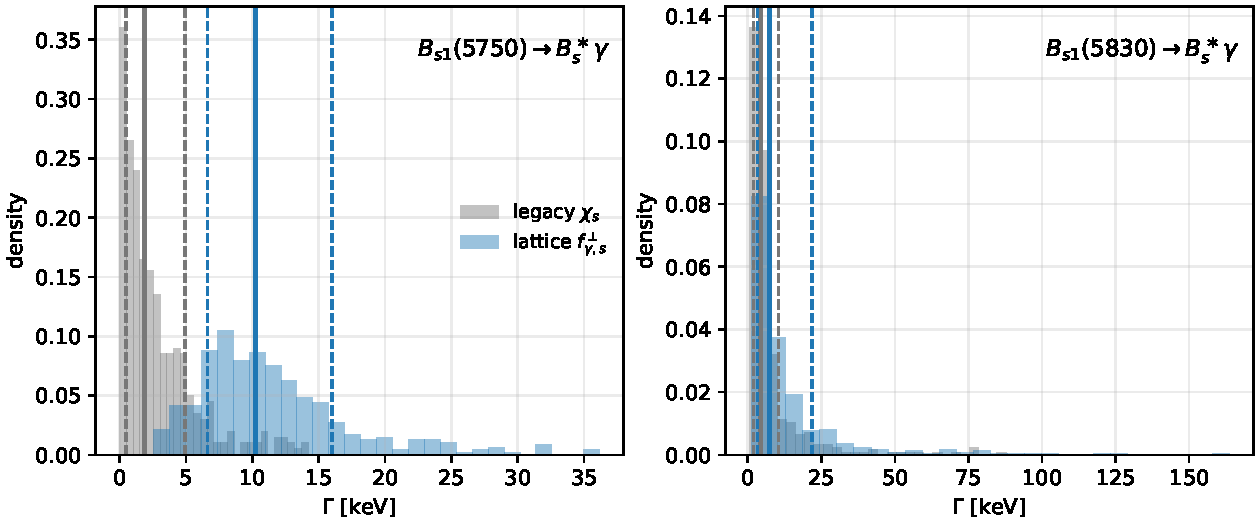
\includegraphics[width=0.48\textwidth]{../Bsstar_gamma/outputs/bsstar_full_calibrated_histograms.pdf}
\caption{Monte Carlo width distributions for the vector-final-state channels.
Left: \(D_{s1}\to D_s^\ast\gamma\).  Right:
\(B_{s1}\to B_s^\ast\gamma\).  The histograms compare the legacy
\(\chi_s\ssbar\) normalization with the preferred lattice
\(\fgammas\) normalization.}
\label{fig:mc-histograms}
\end{figure}

The tensor-current hard piece is numerically subleading but not negligible.
In the charm-strange vector channel one finds
\[
  G_{B,{\rm hard}}^\ast\simeq +0.16 ,
\]
while the soft tensor-current contribution is negative and larger in
magnitude.  The hard term therefore partially reduces the soft tensor-current
effect.  The same calibrated hard-density machinery is used in the bottom
sector after the replacement \(c\to b\).

The uncertainty pattern differs from the pseudoscalar-final-state paper.  In
the old susceptibility-normalized setup the product
\(\chi_s\ssbar\) remains a major normalization uncertainty.  With the lattice
\(\fgammas\) input, the photon normalization uncertainty is reduced.  For
\(\Bsone(5830)\to\Bst\gamma\), the largest uncertainty is instead associated
with the physical-current normalization, especially \(f_2\), because the high
state is cancellation sensitive.  For \(B_{s1}(5750)\to\Bst\gamma\), the
dominant spread tracks the total tensor amplitude, with visible contributions
from \(f_1\), \(f_{\Bst}\), and photon-shape parameters.

\subsection{Comparison with literature and experiment}
\label{subsec:comparison}

Table~\ref{tab:vector-final-literature} compares the present predictions with
representative theoretical results.  The final column summarizes the
experimental status.  It is important that the table does not list a measured
partial width: direct radiative measurements of the vector-final-state modes
are not available at present.

\begin{table}[t]
\centering
\caption{Representative comparison for vector-final-state radiative widths.
Widths are in keV.  The bottom-row ranges collect the values of
Refs.~\cite{Li:2021qgz,Godfrey:2016nwn,Lu:2016bbk}; the other literature
entries are representative values collected in
Refs.~\cite{Godfrey:2005ww,Goity:2000dk,Green:2016occ,Radford:2009bs,
Chen:2020ejk,Korner:1992pz,Bondar:2025smw}.}
\label{tab:vector-final-literature}
\resizebox{\textwidth}{!}{%
\begin{tabular}{lllll}
\toprule
Channel & Earlier theory & Bondar--Milstein & This work & Experimental status\\
\midrule
\(\Dsone(2536)\to\Dst\gamma\)
& \(2.96\)--\(22.8\)
& \(29\)
& \(23.0\,[16.5,35.1]\)
& no direct radiative measurement; \(\Gamma_{\rm tot}=0.92\pm0.05~\MeV\)\\
\(\Dsone(2460)\to\Dst\gamma\)
& \(4.74\)--\(25.1\)
& \(104\)
& \(92.3\,[59.7,138.7]\)
& no direct \(\Dst\gamma\) width; \(D_s\gamma\) and \(\Dst\pi^0\) observed\\
\(B_{s1}(5750)\to\Bst\gamma\)
& \(36.9\)--\(56\)
& \(20\)
& \(10.2\,[6.63,16.24]\)
& no established lower \(B_{s1}\) state or radiative measurement\\
\(\Bsone(5830)\to\Bst\gamma\)
& \(53\)--\(98.8\)
& \(41\)
& \(7.46\,[3.30,24.0]\)
& no direct radiative measurement; observed in \(B^{(*)}K\) spectroscopy\\
\bottomrule
\end{tabular}%
}
\end{table}

The charm-strange values show that our \(\Dsone(2460)\to\Dst\gamma\) width is
close to the large Bondar--Milstein value, while
\(\Dsone(2536)\to\Dst\gamma\) is also in the same tens-of-keV range as their
estimate.  This contrasts with the pseudoscalar-final-state channel, where
the high-state amplitude is much more strongly suppressed.  In our LCSR
language, this difference comes from the different Lorentz structure and the
relative size of the axial and tensor-current basis amplitudes after the
physical-current rotation.

For the bottom-strange channels, our widths are smaller than most quark-model
entries.  This should not be interpreted as a direct conflict with experiment,
because no radiative \(B_{s1}\to\Bst\gamma\) partial width has been measured.
The established \(\Bsone(5830)\) state is observed in \(B^{(*)}K\)
spectroscopy \cite{CMS:2018qdl}, and the lower \(B_{s1}(5750)\) row should be
viewed as a diagnostic prediction for a possible lower axial configuration.

\section{Conclusion}
\label{sec:concl}

We have calculated the vector-final-state radiative transitions
\(\Dsone(2460,2536)\to\Dst\gamma\) and
\(B_{s1}(5750),\Bsone(5830)\to\Bst\gamma\) in light-cone QCD sum rules.  The
calculation uses the same mixed-current convention as the pseudoscalar
analysis, but the final vector current, epsilon Lorentz structure, and width
formula are different.  The axial basis-current sum rule was checked against
the Colangelo pure-current benchmark, and the tensor-current contribution was
included through both soft photon-DA terms and a calibrated hard spectral
density.

With the lattice-normalized strange-photon input and fixed
\(\theta=35.3^\circ\), we obtain
\[
  \Gamma[\Dsone(2460)\to\Dst\gamma]=92.3\,[59.7,138.7]~\keV,
\qquad
  \Gamma[\Dsone(2536)\to\Dst\gamma]=23.0\,[16.5,35.1]~\keV,
\]
and
\[
  \Gamma[B_{s1}(5750)\to\Bst\gamma]=10.2\,[6.63,16.24]~\keV,
\qquad
  \Gamma[\Bsone(5830)\to\Bst\gamma]=7.46\,[3.30,24.0]~\keV.
\]
The \(D_s^\ast\gamma\) results are broadly consistent with the
Bondar--Milstein interference picture, especially for the large
\(\Dsone(2460)\) vector-channel width.  In the bottom-strange sector the
predicted widths are smaller than several quark-model estimates, and direct
radiative measurements are needed to distinguish among the calculations.

The comparison with experiment is presently qualitative.  There are no direct
partial-width measurements for the vector-final-state radiative modes.  The
BaBar and CMS results provide important spectroscopy and total-width context,
but not a direct radiative benchmark.  The predictions given here can therefore
serve as targets for future searches of
\(\Dsone(2536)\to\Dst\gamma\) and
\(\Bsone(5830)\to\Bst\gamma\), and as tests of the spin-mixing structure of
strange heavy axial mesons.

\appendix

\section{Photon DAs and calibrated hard density}
\label{app:details}

The photon distribution amplitudes are used in the BBK/Rohrwild notation
\cite{Ball:2002ps,Rohrwild:2007yt}.  For the leading-twist two-particle DA
we use
\begin{equation}
  \phi_\gamma(u)=6u(1-u).
\end{equation}
The conventional normalization is expressed through
\(\chi_s\ssbar\), while the preferred normalization replaces this product by
the lattice-determined strange photon coupling
\(\fgammas(1~\GeV)=-55.1(1.9)~\MeV\) \cite{Bacchio:2024pij}.  In both
normalizations the same two- and three-particle DA shapes are used.

The hard tensor-current density is obtained by calibrating the FeynCalc
triangle reduction to the known axial hard density.  The axial density is
split into strange-emission and heavy-emission pieces,
\[
  \rho_A^{\rm hard}=\rho_{A,s}^{\rm hard}+\rho_{A,Q}^{\rm hard}.
\]
The tensor density is then reconstructed line by line as in
Eq.~\eqref{eq:calibrated-rho}.  This removes the \(p\cdot q\) and
\(1/(p\cdot q)\) artifacts that cancel in the fully reduced axial expression
and preserves the known logarithmic spectral density as the normalization
benchmark.

\bibliographystyle{apsrev4-2}
\bibliography{../draft_prd/all}

\end{document}
